\documentclass{article}
\usepackage{graphicx} % Required for inserting images
\usepackage{float}
\usepackage[T1]{fontenc}
\usepackage{amsmath}
\usepackage[margin=1in]{geometry}
\usepackage{booktabs}
\usepackage{tabularx}
\usepackage[hidelinks]{hyperref}

\title{Stop cool-off: none vs 1 day vs 5 days vs signal reset}
\author{Experiment report \textperiodcentered{} L/S Gamma Desk, QUANTT}
\date{2026-10-16}

\begin{document}

\maketitle

\textbf{Question:} After a stop, does waiting longer before re-entering the same side (5 trading days, or until the signal resets) beat the live 1-day cool-off on both net P\&L and tail risk?

\textbf{Method:} Pre-registered backtest (experiment \texttt{2026-\allowbreak{}10-\allowbreak{}16-\allowbreak{}stop-\allowbreak{}cooloff}, card committed before any run). Four variants on R2 replay snapshots v1 (config\_hash b040760187f0), development window 2014-06-02 to 2024-12-31, live code, one contract, at 1x and 2x spreads. Costs: \$0.65 per contract, \$0.005 per share, \$1 minimum per order. No stop fired in the 10-year baseline, so every variant uses the same tighter stops, fixed in advance: short stop at 0.5x credit, long stop at 25\% of premium. Variants: \texttt{cool0} (no cool-off), \texttt{cool1} (live rule, the reference), \texttt{cool5} (5 trading days) and \texttt{reset} (no cool-off, but no same-side entry until the signal has left that side; research only). The hold-out (2025-01-01 onward) was not used. This report was written by Claude at the PM's request.

\section{Result vs the pass bar}

The card's first rule is an event floor: if \texttt{cool1} has fewer than 5 stop exits at 1x, the verdict is INCONCLUSIVE. With the tighter stops, \texttt{cool1} had \textbf{3 stops} in ten and a half years. \textbf{The verdict is INCONCLUSIVE (too few events).}

The comparisons below are shown for information only; they do not count. \texttt{cool5} and \texttt{reset} produced exactly the same trades, so they share one column.

\begin{center}\small
\begin{tabularx}{\linewidth}{>{\raggedright\arraybackslash}X >{\raggedright\arraybackslash}X >{\raggedright\arraybackslash}X >{\raggedright\arraybackslash}X}
\toprule
\textbf{Bar} & \textbf{1x} & \textbf{2x} & \textbf{Result} \\
\midrule
Event floor: \texttt{cool1} stops at 1x at least 5 & 3 & (3) & \textbf{fails: INCONCLUSIVE} \\
Net P\&L, full window: \texttt{cool5}/\allowbreak{}\texttt{reset} vs \texttt{cool1} & -\$2,120 vs -\$2,331 & -\$4,289 vs -\$4,540 & higher (info only) \\
Net P\&L, 2014-06 to 2019-12 & -\$1,083 vs -\$1,083 & -\$1,715 vs -\$1,715 & tie, not higher (info only) \\
Net P\&L, 2020-01 to 2024-12 & -\$1,037 vs -\$1,247 & -\$2,574 vs -\$2,825 & higher (info only) \\
ES 5\% (daily), full window & -93.9 vs -98.1 & -102.8 vs -107.1 & less severe (info only) \\
\bottomrule
\end{tabularx}
\end{center}

Even without the event floor the hypothesis would not pass, because the first half is an exact tie. After the only stop in 2014-2019 (August 2015), the 1-day wait was already enough to avoid a same-side re-entry, so \texttt{cool1}, \texttt{cool5} and \texttt{reset} traded the same way until 2020. The whole difference comes from two stops in February and March 2020.

Full-window context at 1x (2x): baseline -\$2,060 (-\$4,122), ES -96.5 (-104.5); \texttt{cool0} -\$2,351 (-\$4,584), ES -100.7 (-110.0); \texttt{cool1} -\$2,331 (-\$4,540), ES -98.1 (-107.1); \texttt{cool5} and \texttt{reset} -\$2,120 (-\$4,289), ES -93.9 (-102.8).

\section{Charts}

\begin{figure}[H]\centering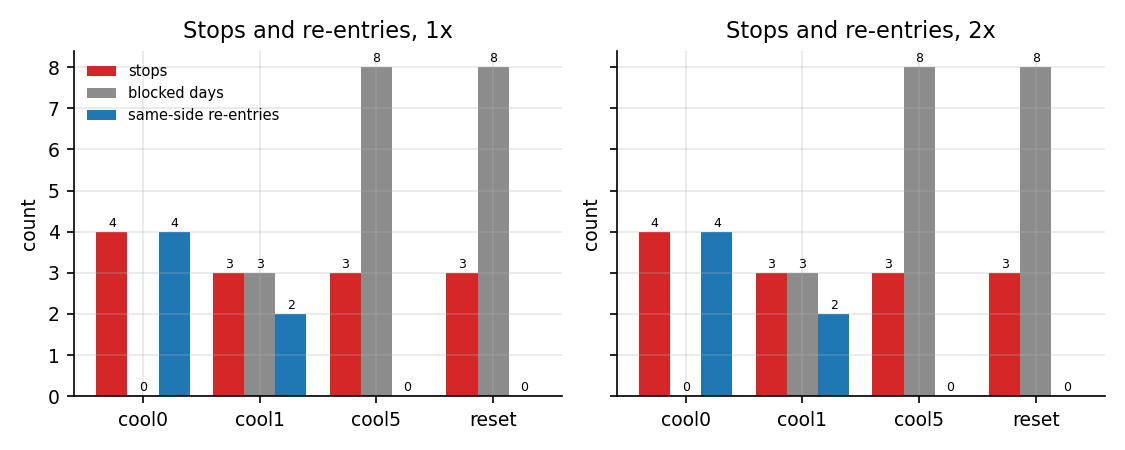
\includegraphics[width=0.92\linewidth]{figures/stops.png}\caption{Stops, blocked days and same-side re-entries per variant}\end{figure}

The tighter stops fired 3 to 4 times. With no cool-off, every stop was followed by a same-side re-entry (4 of 4). The 1-day rule blocked 3 days and still allowed 2 re-entries. Waiting 5 days or for a reset blocked 8 days and allowed none.

\begin{figure}[H]\centering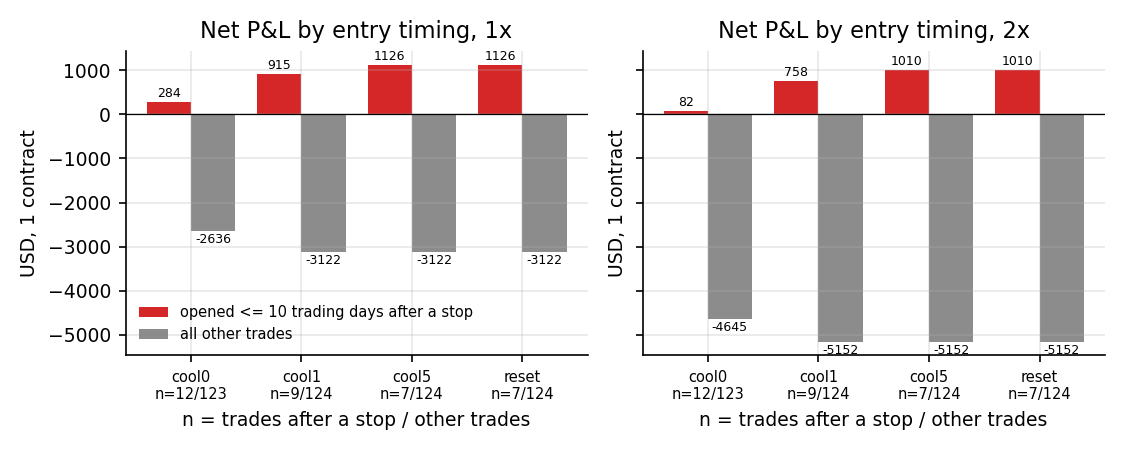
\includegraphics[width=0.92\linewidth]{figures/after_stop.png}\caption{Net P\&L of trades opened within 10 trading days after a stop vs all other trades}\end{figure}

Trades opened soon after a stop made money in every variant, mostly in the 2020 rebound. The one exception is \texttt{cool0}'s longs (\ensuremath{-}\$19 at 1x, \ensuremath{-}\$129 at 2x). Waiting longer raised that group from +\$915 (\texttt{cool1}) to +\$1,126 at 1x. The other trades total the same for \texttt{cool1}, \texttt{cool5} and \texttt{reset} (-\$3,122 at 1x), so the gap between them comes only from the post-stop window. Counts are small (7 to 12 trades).

\begin{figure}[H]\centering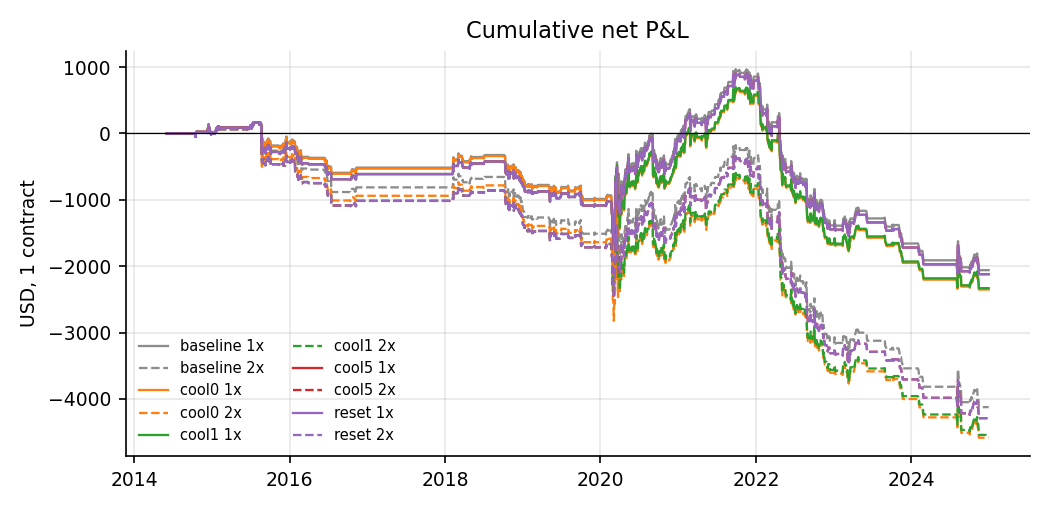
\includegraphics[width=0.92\linewidth]{figures/cum_pnl.png}\caption{Cumulative net P\&L, 1x solid, 2x dashed}\end{figure}

The variants leave the baseline at the August 2015 stop (only \texttt{cool0} re-enters there). \texttt{cool1}, \texttt{cool5} and \texttt{reset} stay together until February 2020, split there, and stay apart by an almost constant amount afterwards. \texttt{cool5} is hidden under \texttt{reset} because the two are identical.

\begin{figure}[H]\centering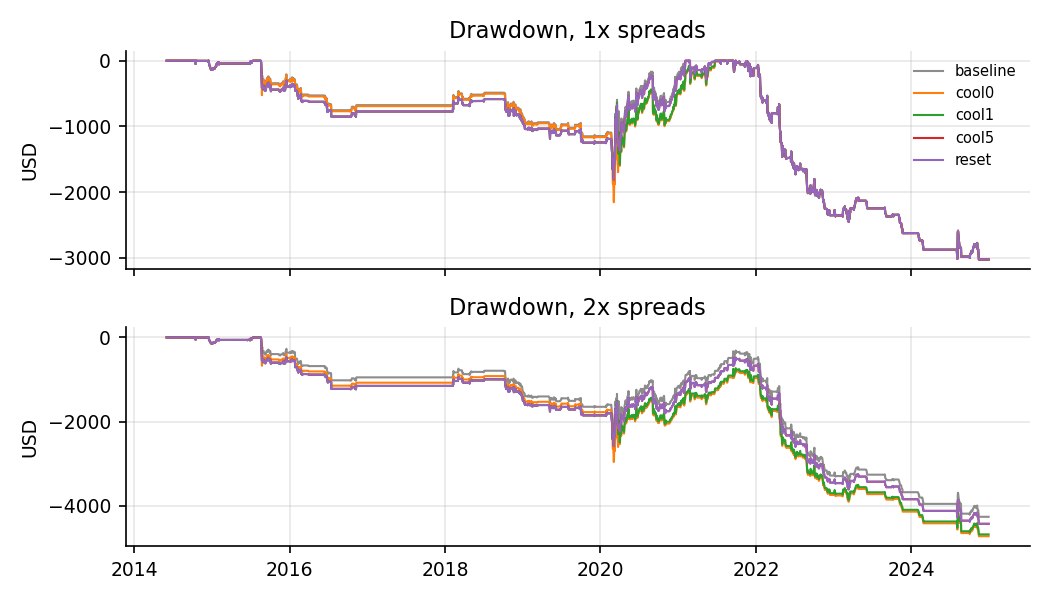
\includegraphics[width=0.92\linewidth]{figures/drawdown.png}\caption{Drawdown at 1x and 2x}\end{figure}

The maximum drawdown is the same for all variants at 1x (\$3,027, reached at the end of 2024). The cool-off rule only changes the depth of the March 2020 dip.

\begin{figure}[H]\centering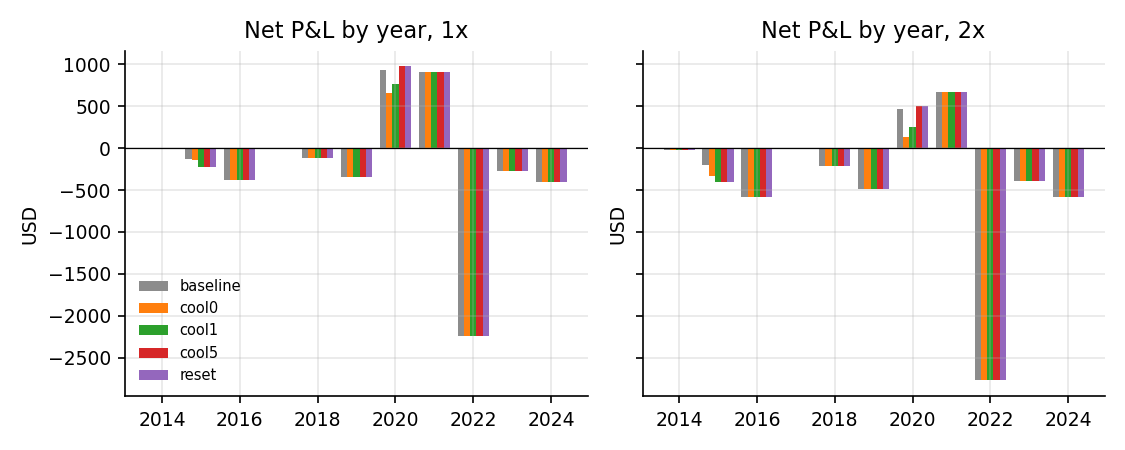
\includegraphics[width=0.92\linewidth]{figures/yearly.png}\caption{Net P\&L by year}\end{figure}

The cool-off rule changes only 2015 and 2020. Waiting longer was better in 2020 and made no difference in 2015.

\begin{figure}[H]\centering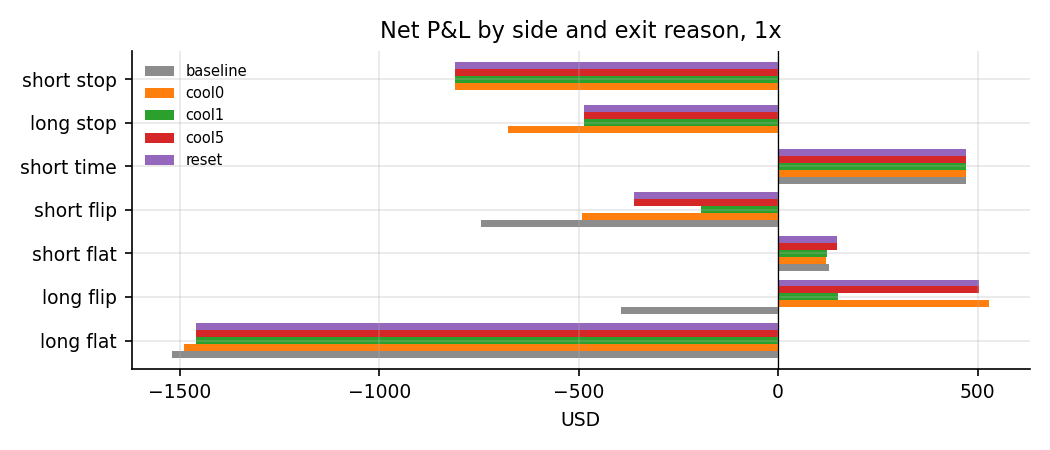
\includegraphics[width=0.92\linewidth]{figures/by_reason.png}\caption{Net P\&L by side and exit reason, 1x}\end{figure}

The stops themselves cost \$1,297 at 1x in \texttt{cool1}, \texttt{cool5} and \texttt{reset}, and \$1,488 in \texttt{cool0} (4 stops). \texttt{cool0} loses more on long stops because it re-entered a long and was stopped again. The longer waits gain mainly on long flips.

\begin{figure}[H]\centering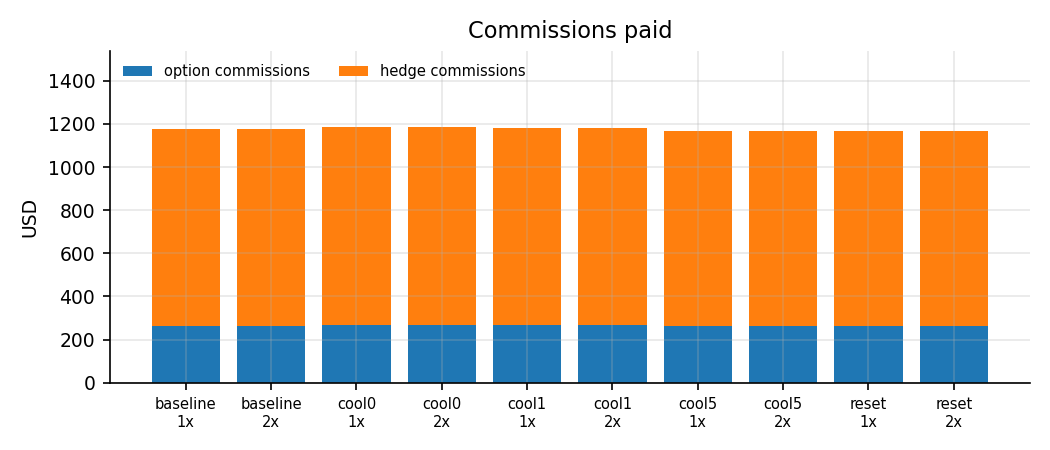
\includegraphics[width=0.92\linewidth]{figures/fees.png}\caption{Commissions paid}\end{figure}

Commissions are almost the same in every variant (about \$1,170). Hedge orders and their \$1 minimum dominate, so the cool-off rule has no meaningful effect on costs.

\section{Analysis}

The test could not answer its question, because the tighter stops fired only 3 times in ten and a half years: a short in August 2015, then a short in February 2020 and a long in March 2020. The two 2020 stops drive all the differences between the variants. The full-window direction is the one the hypothesis predicted (more P\&L and a less severe ES at both spreads for the longer waits), but the mechanism is not the clean one the hypothesis assumed. The 1-day rule's two same-side re-entries in 2020 lost only \$47 in total, and with no cool-off the four immediate re-entries made \$169. Most of the \$210 gain from waiting comes from path dependence: skipping the re-entry changed which trades came next during the 2020 rebound (mainly a better long flip). One crash and a different sequence of later trades is not evidence that waiting is better in general, and the first half shows no difference at all.

\texttt{cool5} and \texttt{reset} were identical: in each of the three episodes the two rules blocked the same 8 days and allowed the same next trade. On this data they cannot be told apart.

None of the variants beats the baseline (live stops, which never fired) at 1x: the tighter stops cost money no matter what cool-off follows them. The cool-off result is therefore conditional on stops that the desk does not run live; experiment \texttt{2026-\allowbreak{}10-\allowbreak{}16-\allowbreak{}stop-\allowbreak{}levels} tests the stop levels themselves.

\section{Verdict}

\textbf{INCONCLUSIVE (too few events).} \texttt{cool1} had 3 stop exits at 1x, below the pre-registered floor of 5. The live rule (\texttt{[exit] stop\_\allowbreak{}cooloff\_\allowbreak{}days = 1}) stays. The 2020 episode points towards a longer wait, but it rests on one crash and on path effects rather than on losing re-entries, and even without the floor the first-half tie would have failed the bar. A useful follow-up needs more stop events: more symbols (the R2 bucket also has QQQ and IWM options), or a stop level that fires more often. Any such test would need its own card.

\section{Caveats}

\begin{itemize}

\item \textbf{In-sample idea:} the need for this test, and the tighter stops, came from the baseline on the same window. Even a pass would have needed one hold-out run.

\item \textbf{Tiny sample:} 3 stops, 2 of them in one crash, and 7 to 12 trades after a stop. The comparison rests on a handful of trades.

\item \textbf{Conditional on tighter stops:} the live stops never fired, so the cool-off rule has had no effect on the live configuration in ten years.

\item \textbf{One contract:} the \$1 minimum per order is large relative to the position size. It dominates hedge costs, the same in every variant.

\item \textbf{Spread model:} half-spreads are fitted on about two weeks of calm 2026 live quotes. They are probably too narrow in crashes, which is exactly when the stops fire.

\item \textbf{Missing data:} month-end R2 days are missing; 3.3\% of scheduled times were skipped.

\item \textbf{Weekdays:} cool-off days are counted as weekdays, as in the live rule, so an exchange holiday counts as a day.

\end{itemize}

\section{Trials}

This experiment registered 8 trials (4 variants at 1x and 2x), run once on commit 8d1f0fe, with the pass bar committed before the run. Adding the baseline's 2 trials gives 10. The baseline regression check that reproduced trial 1 was not registered. \texttt{cool1} has exactly the same configuration as the \texttt{tight} variant of \texttt{2026-\allowbreak{}10-\allowbreak{}16-\allowbreak{}stop-\allowbreak{}levels}, and its results reproduce that experiment's numbers exactly (-\$2,330.67 and ES -98.06 at 1x). It is a duplicate trial, accepted in advance by the PM. Some registry rows are marked ``dirty'' because other experiments' uncommitted research files were in the working tree during the run; this experiment's script, the configs and \texttt{src/\allowbreak{}} were unchanged from 8d1f0fe.

\end{document}
